 \documentclass[12pt]{article}
\usepackage[top=1in, bottom=1in, left=1.25in, right=1.25in]{geometry}
\usepackage{float}
\usepackage{color}
\usepackage{amssymb}
\usepackage{amsthm}
\usepackage{multirow}
%
%\newtheorem*{remark}{Remark}
\usepackage[round]{natbib}
\usepackage{algorithm}
%\usepackage{setspace}
\usepackage{amsmath}
\usepackage{graphicx}
\usepackage{caption}
\usepackage{bm}
\usepackage[pdftex,hypertexnames=false,linktocpage=true]{hyperref}
\hypersetup{colorlinks=true,linkcolor=blue,anchorcolor=blue,citecolor=blue,filecolor=blue,urlcolor=blue,bookmarksnumbered=true,pdfview=FitB}
\providecommand{\keywords}[1]{\textbf{\textit{Key words:}} #1}

\def\T{{ \mathrm{\scriptscriptstyle T} }}
\def\v{{\varepsilon}}

\def\pr{{\rm pr}}
\def\E{{\rm E}}
\def\V{{\rm Var}}

\def\0{{\bf 0}}
\def\A{{\bf A}}
\def\ua{{\bf a}}
\def\uB{{\bf B}}
\def\ub{{\bf b}}
\def\C{{\bf C}}
\def\c{{\bf c}}
\def\uD{{\bf D}}
\def\ud{{\bf d}}
\def\ue{{\bf e}}
\def\uE{{\bf E}}
\def\f{{\bf f}}
\def\h{{\bf h}}
\def\g{{\bf g}}
\def\uI{{\bf I}}
\def\K{{\bf K}}
\def\um{{\bf m}}
\def\uM{{\bf M}}
\def\r{{\bf r}}
\def\t{{\bf t}}
\def\T{{\bf T}}
\def\bO{{\bf O}}
\def\bP{{\bf P}}
\def\uQ{{\bf Q}}
\def\U{{\bf U}}
\def\uv{{\bf v}}
\def\uV{{\bf V}}
\def\uS{{\bf S}}
\def\uu{{\bf u}}
\def\uW{{\bf W}}
\def\uH{{\bf H}}
\def\uX{{\bf X}}
\def\ux{{\bf x}}

\def\uY{{\bf Y}}
\def\uy{{\bf y}}
\def\Z{{\bf Z}}
\def\uz{{\bf z}}

\def\0{{\boldsymbol 0}}
\def\1{{\boldsymbol 1}}
\def\ubeta{{\boldsymbol \beta}}
\def\btau{{\boldsymbol \tau}}
\def\bg{{\boldsymbol \gamma}}
\def\ueta{{\boldsymbol \eta}}
\def\bpi{{\boldsymbol \pi}}
\def\uxi{{\boldsymbol \xi}}
\def\ueta{{\boldsymbol \eta}}
\def\utheta{{\boldsymbol \theta}}
\def\umu{{\boldsymbol \mu}}
\def\uepsilon{{\boldsymbol \epsilon}}
\def\bOmega{{\boldsymbol\Omega}}
\def\uSigma{{\boldsymbol \Sigma}}
\def\bLam{{\bf \Lambda}}
\def\T{{ \mathrm{\scriptscriptstyle T} }}
\def\ualpha{{\boldsymbol \alpha}}
\def\usigma{{\boldsymbol \sigma}}
\def\uphi{{\boldsymbol \phi}}
\def\uepsilon{{\boldsymbol \epsilon}}
\def\nbd{{\rm nbd}}
\def\diag{{\rm diag}}


\def\T{{ \mathrm{\scriptscriptstyle T} }}


\newtheorem{theorem}{Theorem}
\newtheorem{lemma}{Lemma}
\newtheorem{proposition}{Proposition}
\newtheorem{corollary}{Corollary}
\newtheorem{definition}{Definition}
\newtheorem{remark}{Remark}
\newtheorem{example}{Example}
\newtheorem{assumption}{Assumption}

% newcommand used in the document

%opening
\title{\LARGE\bf Bayesian selection of best subsets in high-dimensional regression}
\author{ Shiqiang Jin\thanks{Department of Statistics, Kansas State University, Manhattan, KS 66506, U.S.A.} \and Gyuhyeong Goh\thanks{Department of Statistics, Kansas State University, Manhattan, KS 66506, U.S.A.} }

\begin{document}
\baselineskip .3in
\maketitle

\begin{abstract}
With large numbers of predictors, regression analysis has faced many challenges including model fitting and prediction. As a power tool for dimension reduction, high-dimensional variable selection has drawn increasing attention in recent years. In this paper, we develop a new Bayesian approach to best subset selection that quickly identifies the best subset from a high-dimensional set of candidates via a hybrid search algorithm of deterministic local search and stochastic global search. To reduce the computational cost of evaluating many candidate subsets needed for each iteration, we propose an efficient and fast computation strategy that enables us to calculate exact posterior probabilities of all neighbor models simultaneously. The proposed Bayesian method possesses model selection consistency in the high-dimensional setting in which the number of candidate predictors is allowed to grow faster than the sample size. Simulation study and real data analysis are performed to assess and validate the proposed method.
\end{abstract}

\keywords{Bayesian subset selection}

\section{Introduction}
Variable selection plays a key role in recent regression analysis. In many statistical applications, especially in genetics studies, researchers have faced the situation in which the number of candidate predictors is extremely large but the sample size is relatively small, often referred to as a high-dimensional regression problem. The most pressing challenge in high-dimensional regression is to identify relevant predictor variables from the huge pool of candidates. In an attempt to perform high-dimensional variable selection, a lot of effort has been put into the development of penalized likelihood methods (e.g., \citealt{tibshirani1996regression, fan2001variable, zou2005regularization, zhang2010nearly}). By adding a penalty function to the likelihood criterion, a penalized likelihood method produces sparse solutions that eliminate irrelevant predictors corresponding to the zero-estimated coefficients in the regression model. 

In this paper, we are interested in selecting $k$ important predictors out of $p$ candidates, called the best subset selection problem \citep{hocking1967selection}. It is well known that the best subset selection involves non-convex optimization, which is computationally intractable in high-dimensional settings (i.e., when $p$ is large). Although some penalized likelihood approaches such as Lasso, elastic net, and MCP provide a convex surrogate for the non-convex optimization problem, their applicability to the best subset selection is still limited \citep{bertsimas2016best}. Recently, a Bayesian approach to best subset selection, called Bayesian subset regression (BSR), has been proposed by \citet{liang2013bayesian}. Using an adaptive Markov chain Monte Carlo (MCMC) algorithm, called the stochastic approximation Monte Carlo \citep{liang2007stochastic}, BSR finds the best subset by performing a global search over the entire model space. However, the global stochastic search with a large number of candidate predictors often raises computational challenges including heavy computation and slow convergence. To overcome this limitation, we introduce new Bayesian subset selection algorithms that quickly identify the best subset via hybrid algorithms of deterministic local search and stochastic global search. The main attractive feature of our proposed method is that evaluating all possible candidate models for the next update, which is the most expensive part of MCMC computation, is simultaneously accomplished.

%The rest of the paper is organized as follows. In Section \ref{sec:2}, we describe the model setup and assumptions. In Section \ref{sec:3}, we extend the proposed method to variable selection. \textcolor{red}{In section \ref{sec:4}, we prove our algorithm obtains local optimization analytically but tends to target global optimized solution in numerical way.} In Section \ref{sec:5}, by using a simulation study, our proposed method is compared with some commonly used variable selection approaches including LASSO, SCAD, MCP and EMVS. The simulation result clear shows many benefits of our method. In Section \ref{sec:6}, we perform real data analysis with gene expression data. Section \ref{sec:7} concludes our paper with some remarks. The rest of the paper is organized as follows. Section 2 describes some explicit calculations to obtain a closed-form of In Section 3, we introduce a new Bayesian variable selection procedure via the ICM algorithm and discuss its important features. In Section 4, we study the performance of the newly-developed Bayesian variable method on simulated high-dimensional data. Section 6 offers some concluding remarks.

%In this paper, we denote normal distribution and inverse gamma distribution by $\mathcal{N}$ and $\mathcal{IG}$.

\section{Basic setup}\label{sec:2}
Consider a multiple linear regression model,
\begin{eqnarray}\label{eq:1}
\uy = \uX\ubeta + \uepsilon,
\end{eqnarray}
where $\uy$ is the $n$-dimensional response vector, $\uX = (\ux_1,\ldots,\ux_p)$ is the $n\times p$ design matrix, $\ubeta = (\beta_1,\ldots,\beta_p)^{\T}$ is a $p$-dimensional coefficient vector, and $\uepsilon \sim\text{Normal}(\0_n, \sigma^2\uI_n)$. As we are interested in high-dimensional problems, we assume that $p>n$ and $\ubeta$ contains many zero elements, i.e., $\ubeta$ is a high-dimensional sparse vector. We further assume that the response and predictors are standardized so that the intercept is always excluded from our regression analysis. Here, our goal is to identify the most important $k$ predictors in \eqref{eq:1}. To this end, let $\bg=(\gamma_1,\ldots,\gamma_p)$ be a vector of binary variables such that $\gamma_j=1$ if the $j^{th}$ predictor, $\ux_j$, is active and $\gamma_j=0$ otherwise for $j=1,\ldots,p$. For a given $\bg$, we can reduce the model \eqref{eq:1} to
\begin{eqnarray*}
\uy = \uX_{\bg} \ubeta_{\bg} + \uepsilon,
\end{eqnarray*}
where $\uX_{\bg}$ and $\ubeta_{\bg}$ are a sub-matrix of $\uX$ and a sub-vector of $\ubeta$ corresponding to the non-zero elements of $\bg$, respectively. Given $\bg$, we assign conjugate priors for $\ubeta_{\bg}$ and $\sigma^2$ that are most commonly used in Bayesian linear regression,
\begin{eqnarray*}
	\ubeta_{\bg}|\sigma^2,\bg &\sim&\text{Normal}(0,\tau \sigma^2 \uI_{|\bg|} ),\\
	\sigma^2 &\sim& \text{Inverse-Gamma}(a_{\sigma}/2,b_{\sigma}/2),
\end{eqnarray*} 
where $\tau$, $a_{\sigma}$, and $b_{\sigma}$ denote hyperparameters and $|\bg|=\sum_{j=1}^p\gamma_j $ indicates the number of active predictors in the reduced model. To impose the constraint $|\bg|=k$, we define the prior distribution of $\bg$ by $\pi(\bg)\propto\mathbb{I}(|\bg|=k )$, where $\mathbb{I}(\cdot)$ is an indicator function. Let $m(\uy|\bg)$ be the marginal likelihood given $\bg$. Using the kernels of normal density and inverse gamma density, the marginal likelihood can be easily calculated as
\begin{eqnarray}
\nonumber m(\uy|\bg) &=&\int f(\uy|\ubeta_{\bg},\sigma^2)\pi(\ubeta_{\bg}|\sigma^2, \bg) \pi(\sigma^2) d\ubeta d\sigma^2\\
\label{eq:2}&\propto& \frac{(\tau^{-1})^{\frac{|\bg|}{2}}}{|\uX_{\bg}^{\T}
		\uX_{\bg}+\tau^{-1}\uI_{|\bg|} |^{\frac{1}{2}}  \left(\uy^{\T}\uH_{\bg}
	\uy+b_{\sigma}\right)^{\frac{a_{\sigma}+n}{2}  } },
\end{eqnarray}
where $f(\uy|\ubeta_{\bg},\sigma^2)$ denotes the likelihood given $\bg$ and $\uH_{\bg} = \uI_n-\uX_{\bg}(\uX_{\bg}^{\T}\uX_{\bg}+\tau^{-1}\uI_{|\bg|})^{-1}\uX_{\bg}^{\T}$. By Bayes' theorem, the posterior model probability of $\bg$ is proportional to $$\pi(\bg|\uy)\propto m(\uy|\bg) \pi(\bg) \propto  \frac{(\tau^{-1})^{\frac{|\bg|}{2}}}{|\uX_{\bg}^{\T}
		\uX_{\bg}+\tau^{-1}\uI_{|\bg|} |^{\frac{1}{2}}  \left(\uy^{\T}\uH_{\bg}
	\uy+b_{\sigma}\right)^{\frac{a_{\sigma}+n}{2}  } } \mathbb{I}(|\bg|=k ):=Q(\bg).$$
Therefore, our Bayesian best subset selection can be achieved by maximizing $Q(\bg)$.
\section{Best subset selection with fixed-size}
In this section, we introduce new algorithms to reach at $\hat{\bg}=\arg\max_{\bg}\pi(\bg|\uy)$ for the fixed subset size, $k$. Let $\mathcal{N}_+(\bg)$ be the set of all larger neighbors of $\bg$ obtained by adding one new predictor variable to $\bg$. Similarly, let $\mathcal{N}_-(\bg)$ be the set of all smaller neighbors of $\bg$ obtained by deleting one variable from $\bg$. Suppose that $\tilde{\bg}$ represents the current best subset of size $k$. Our main idea is to update $\tilde{\bg}$ via the following two-step procedure until convergence:
\begin{itemize}
\item[] \textbf{Addition-step:} Using the marginal likelihood, \emph{evaluate all models} in $\mathcal{N}_+(\tilde{\bg})$ \emph{simultaneously} and then find the best subset of size $k+1$, $$\tilde{\ueta}=\arg\max_{\ueta  \in \mathcal{N}_+(\tilde{\bg} ) } m(\uy|\ueta).$$
\item[] \textbf{Deletion-step:} Using the marginal likelihood, \emph{evaluate all models} in $\mathcal{N}_-(\tilde{\ueta})$ \emph{simultaneously} and then update the best subset of size $k$ as
$$\tilde{\bg}= \arg\max_{\bg  \in \mathcal{N}_-(\tilde{\ueta} ) } m(\uy|\bg).$$
\end{itemize}
The following theorem proves the convergence of the proposed algorithm.
\begin{theorem}\label{thm:1} The proposed algorithm monotonically increases the posterior probability, $\pi(\tilde{\bg}|\uy)$. In addition, the algorithm terminates in a finite number of iterations.
\end{theorem}
The proof is given in Appendix \ref{app:01}. The great merit of our approach is that evaluating all the candidates for each step can be done simultaneously. To explain this in more details, let $\mathcal{G}_0=\{i:\tilde{\gamma}_i=0\}$ be an index set of inactive predictors associated with $\tilde{\bg}$, where $\tilde{\gamma}_i$ is the $i^{th}$ element of $\tilde{\bg}$. For each $i\in \mathcal{G}_0$, define $\ueta_i=(\eta_{i1},\ldots,\eta_{ip})$ by replacing the $i^{th}$ element of $\tilde{\bg}$ with $1$, that is, $\eta_{ij}=1$ if $j=i$ and $\eta_{ij}=\tilde{\gamma}_j$ if $j\neq i$. For every $i\in \mathcal{G}_0$, using \eqref{eq:2}, it can be shown that
\begin{eqnarray}\label{eq:app:1}
 m(\uy|\ueta_i) \propto \left[\uy^{\T}\uH_{\tilde{\bg}}\uy-\frac{(
 	\ux_i^{\T}\uH_{\tilde{\bg}}\uy)^2}{\tau^{-1}+\ux_i^{\T}\uH_{\tilde{\bg}} \ux_i }+b_{\sigma}\right]^
 {-\frac{a_{\sigma}+n}{2}}(\tau^{-1}+\ux_i^{\T}\uH_{\tilde{\bg}} \ux_i)^{-1/2},
\end{eqnarray}
where $\ux_i$ is the $i^{th}$ column of $\uX$. The details of our calculation in \eqref{eq:app:1} are shown by Appendix \ref{app:1}. It is important to note that $\ux_i^{\T}\uH_{\tilde{\bg}}\ux_i$ is the $i^{th}$ diagonal element of $\uX^{\T}\uH_{\tilde{\bg}}\uX$ and that $\ux_i^{\T}\uH_{\tilde{\bg}}\uy$ is the $i^{th}$ element of $\uX^{\T}\uH_{\tilde{\bg}}\uy$. Let $s_{\tilde{\bg}}=\uy^{\T}\uH_{\tilde{\bg}}\uy$, $\ud_{\tilde{\bg}}=\diag(\uX^{\T}\uH_{\tilde{\bg}}\uX)$, and $\uv_{\tilde{\bg}}=\uX^{\T}\uH_{\tilde{\bg}}\uy$. Define
$$\um^+_{\tilde{\bg}}= \left[(s_{\tilde{\bg}}+b_{\sigma}) \1_p-\frac{\uv_{\tilde{\bg}}^2}{\tau^{-1}\1_p+\ud_{\tilde{\bg}} } \right]^
 {-\frac{a_{\sigma}+n}{2}}(\tau^{-1} \1_p  +\ud_{\tilde{\bg}} )^{-1/2},$$
 where $\ua^x=(a_1^x,\ldots, a_p^x)$ and $\ua/\ub=(a_1/b_1,\ldots,a_p/b_p)$ for generic vectors $\ua$ and $\ub$. Note that $\mathcal{N}_+(\tilde{\bg})=\{\ueta_i:i\in \mathcal{G}_0\}$. Hence, in the addition-step, evaluating all the models in $\mathcal{N}_+(\tilde{\bg})$ (i.e.,  calculating all the marginal likelihoods) can be done at once by extracting the sub-vector corresponding to $\mathcal{G}_0$ from $\um^+_{\tilde{\bg}}$. Similarly, let $\mathcal{E}_1=\{\ell:\tilde{\eta}_\ell=1\}$ be an index set of active predictors associated with $\tilde{\ueta}$, where $\tilde{\eta}_\ell$ denotes the $\ell^{th}$ element of $\tilde{\ueta}$. For each $\ell \in\mathcal{E}_1$, we define $\bg_\ell$ by replacing the $\ell^{th}$ element of $\tilde{\ueta}$ with $0$. We can show that 
 \begin{eqnarray}\label{eq:app:2}
 m(\uy|\bg_\ell)  \propto \left[\uy^{\T}\uH_{\tilde{\ueta}}\uy+\frac{(
 	\ux_\ell^{\T}\uH_{\tilde{\ueta}}\uy)^2}{\tau^{-1}-\ux_\ell^{\T}\uH_{\tilde{\ueta}} \ux_\ell }+b_{\sigma}\right]^
 {-\frac{a_{\sigma}+n}{2}}(\tau^{-1}-\ux_\ell^{\T}\uH_{\tilde{\ueta}} \ux_\ell)^{-1/2}.
\end{eqnarray} Some details of our calculation for \eqref{eq:app:2} are shown in Appendix \ref{app:2}. Define
$$\um^-_{\tilde{\ueta}}= \left[(s_{\tilde{\ueta}}+b_{\sigma}) \1_p+\frac{\uv_{\tilde{\ueta}}^2}{\tau^{-1}\1_p-\ud_{\tilde{\ueta}} } \right]^
 {-\frac{a_{\sigma}+n}{2}}(\tau^{-1} \1_p  -\ud_{\tilde{\ueta}} )^{-1/2}.$$
Note that $\mathcal{N}_-(\tilde{\ueta})=\{\bg_\ell:\ell\in \mathcal{E}_1\}$. Hence, as in the addition-step,  evaluating all the candidates in the deletion-step can be done at once by extracting the sub-vector corresponding to $\mathcal{E}_1$ from $\um^-_{\tilde{\ueta}}$. 

In general, hyperparameter $\tau$ can be chosen to be a large value so that the Gaussian prior for $\ubeta_{\bg}$ becomes approximately non-informative (or flat). However, when predictors are strongly correlated (i.e., when multicollinearity occurs), hyperparameter optimization for $\tau$ plays a crucial role to improve the prediction accuracy \citep{hoerl1970ridge}. Since multicollinearly is common in high-dimensional settings, we propose to estimate the optimal value of $\tau$ using an empirical Bayesian approach. Note that, given $\bg$, the marginal likelihood in \eqref{eq:2} can be considered as a function of $\tau$. Taking the negative logarithm of the right hand side of $\eqref{eq:2}$ and applying Lemma \ref{lem:1} in Appendix \ref{app:3}, we define
\begin{eqnarray}
	\nonumber Q(\tau|\bg) 
	&=&\frac{|\bg|}{2}\log\tau+ \frac{1}{2}\sum_{j=1}^{p}\log  (\lambda_{\bg j} +\tau^{-1})\\
	\label{gtau} && + {\frac{a_{\sigma}+n}{2}}\log\left\{\uy^{\T}\uy 
	-\sum_{j=1}^p \frac{\lambda_{\bg j} (\uu_{\bg j}^\T \uy)^2}{\lambda_{\bg j}+\tau^{-1} }+b_{\sigma} \right\},
\end{eqnarray}
where $\lambda_{\bg j}$ is the $j^{th}$ largest eigenvalue of $\uX_\bg^\T \uX_\bg$ and $\uu_{\bg j}$ is the eigenvector of $\uX_\bg^\T \uX_\bg$ corresponding to $\lambda_{\bg j}$. Then, for given $\tilde{\bg}$, we estimate the optimal value of $\tau$, say $\tilde{\tau}$, by minimizing $Q(\tau|\tilde{\bg})$. Note that $\tilde{\tau}$ can be easily and quickly obtained by using a simple numerical optimization method such as the Newton-Raphson method. We now introduce our Bayesian best subset algorithm as follows:
\begin{algorithm}[ht]
\caption{Deterministic best subset search with a fixed $k$}\label{alg:1}
\begin{itemize}
\item[1.] Initialize $\tilde{\bg}$ and $\tilde{\tau}$.
\item[2.] \textbf{Repeat}
\begin{itemize}
\item[] Update $\tilde{\ueta}\leftarrow \arg\max_{\ueta  \in \mathcal{N}_+(\tilde{\bg} ) } m(\uy|\ueta,\tilde{\tau})$; 
\item[] Update $\tilde{\bg}\leftarrow  \arg\max_{\bg  \in \mathcal{N}_-(\tilde{\ueta} ) } m(\uy|\bg,\tilde{\tau})$;
\item[] Update $\tilde{\tau} \leftarrow \arg\min_{\tau \in (0,\infty)}Q(\tau|\tilde{\bg})$;
\end{itemize}
\item[] \textbf{until} convergence.
\item[3.] Return $\hat{\bg}=\tilde{\bg}$.
\end{itemize}
\end{algorithm}

A possible drawback of our deterministic search is that the proposed algorithm can get trapped in a local optimum. To resolve this issue, we propose to add a stochastic global search algorithm to the proposed deterministic local search algorithm. This additional step will be used only to check whether or not the local search algorithm reaches the global optimum. To develop a fast global search algorithm, we employ a notion of the shotgun stochastic search \citep{hans2007shotgun}. However, while the shotgun stochastic search evaluates the candidate models using parallel computing, our simultaneous evaluation is based on analytical calculations. Our stochastic search algorithm can be implemented by generating a Markov chain via the following iterative sampling scheme:
\begin{itemize}
\item[1.] Given $\bg^*$, generate $\ueta^*$ with probability,
$$\pi(\ueta|\uy,\bg^*)=\frac{m(\uy|\ueta)}{\sum_{\ueta \in \mathcal{N}_+(\bg^* )  } m(\uy|\ueta) }\mathbb{I}\{\ueta \in \mathcal{N}_+(\bg^* ) \}.$$
\item[2.] Given $\ueta^*$, generate $\bg^*$ with probability
$$\pi(\bg|\uy,\ueta^*)=\frac{m(\uy|\bg)}{\sum_{\bg \in \mathcal{N}_-({\ueta}^* )  } m(\uy|\bg) }\mathbb{I}\{\bg \in \mathcal{N}_-({\ueta}^* )   \}.$$
\end{itemize}
Recall that  using $\eqref{eq:app:1}$ and  $\eqref{eq:app:2}$, calculating $\pi(\ueta|\uy,\bg^*)$ for all $\ueta \in \mathcal{N}_+(\bg^* )$ can be done simultaneously. Similarly, we can calculate $\pi(\bg|\uy,\ueta^*)$ for all $\bg \in \mathcal{N}_-({\ueta}^* ) $ at once.   
Using the notion of the Metropolis-Hasting algorithm, it is easy to check that the states of generated Markov chain by our sampling method is equivalent to the support of $\pi(\bg|\uy)$\textcolor{red}{(Revise it later)}. Let $\bg^{(t)}$ be the sample generated at iteration $t$. If the outcome from Algorithm \ref{alg:1}, $\hat{\bg}$, is not the global maximum, then we must observe at least one case that $\pi(\hat{\bg}|\uy)< \pi(\bg^{(t)}|\uy)$ (or equivalently $m(\uy|\hat{\bg})<m(\uy|\bg^{(t)})$) with probability one as $t\to \infty$. Therefore, if this case does not occur for sufficiently large $t$, we can treat $\hat{\bg}$ as the global maximum.

\begin{algorithm}[ht]
\caption{Hybrid best subset search with a fixed $k$}\label{alg:2}
\begin{itemize}
\item[1.] Initialize $\tilde{\bg}$ and $\tilde{\tau}$.
\item[2.] \textbf{Repeat}
\begin{itemize}
\item[] Update $\tilde{\ueta}\leftarrow \arg\max_{\ueta  \in \mathcal{N}_+(\tilde{\bg} ) } m(\uy|\ueta,\tilde{\tau});$ 
\item[] Update $\tilde{\bg}\leftarrow  \arg\max_{\bg  \in \mathcal{N}_-(\tilde{\ueta} ) } m(\uy|\bg,\tilde{\tau});$
\item[] Update $\tilde{\tau} \leftarrow \arg\min_{\tau \in (0,\infty)}Q(\tau|\tilde{\bg})$;
\end{itemize}
\item[] \textbf{until} convergence.
\item[3.] Set $\bg^{(0)}=\tilde{\bg}$.
\item[4.] \textbf{Repeat} for $t=1,\ldots,T$:
\begin{itemize}
\item[] Generate $\ueta^{(t)}\sim \pi(\ueta|\uy,\bg^{(t-1)})$;
\item[] Generate $\bg^{(t)}\sim \pi(\bg|\uy,\ueta^{(t)})$;
\item[] \textbf{If} $m(\uy|\tilde{\bg})<m(\uy|\bg^{(t)})$, \textbf{then} set $\tilde{\bg}=\bg^{(t)}$, break the loop, and go to 2.
\end{itemize}
\item[5.] Return $\hat{\bg}=\tilde{\bg}$.
\end{itemize}
\end{algorithm}

\section{Best subset selection with bounded size}\label{sec:3}
In this section, we extend the proposed method to best subset selection with varying $k (\leq K)$ for a prespecified upper bound $K$, which is a common setting for high-dimensional best subset selection (e.g., \citealt{bertsimas2016best, liang2013bayesian}). In our Bayesian framework, this extension can be easily done by assigning an appropriate prior for unknown $k$. As a non-informative prior, one may consider a discrete uniform prior for $k$, that is, $k \sim \text{Uniform}\{1,\ldots,K\}$. However, the uniform prior tends to assign larger probability to a larger subset due to the fact that the total number of subsets is $\binom{p}{k}$ for $k$. To remove this issue, using  a similar idea of \citet{chen2008extended}, we define 
$$\pi(k)\propto 1/\binom{p}{k} \mathbb{I}(k\leq K).$$
Let $\bg_{k}=(\gamma_{k1},\ldots,\gamma_{kp})$ indicate a subset of size $k$. Then, our best subset selection can be performed by maximizing  
\begin{eqnarray*}
\pi(\bg_k|\uy)\propto  m(\uy|\bg_k)/\binom{p}{k},
\end{eqnarray*}
subject to $k\leq K$. Hence, our best subset search algorithms with varying $k$ can be summarized as follows:
\begin{algorithm}[ht]
\caption{Best subset search with varying $k$}\label{alg:3}
\begin{itemize}
\item[1.] \textbf{Repeat} for $k=1,\ldots,K$:
\begin{itemize}
\item[a.] Initialize $\tilde{\bg}$ and $\tilde{\tau}$.
\item[b.] Implement step 2 of Algorithm \ref{alg:1} for deterministic search.
\item[] (or Implement steps 2 -- 4 of Algorithm \ref{alg:2} for hybrid search.)
\item[c.] Set $\hat{\bg}_k=\tilde{\bg}$.
\end{itemize}
\item[2.] Return $\hat{\bg}=\hat{\bg}_{\hat{k}}$, where \begin{eqnarray}\label{eq:post}  \hat{k}=\arg\max_{1\leq k\leq K} \left\{\log m(\uy|\hat{\bg}_k)-\log \binom{p}{k}\right\}.
\end{eqnarray}
\end{itemize}
\end{algorithm}

From \citet{kass1995}, for sufficiently large $n$, we have 
$$  \log m(\uy|\bg_{k_1}) -\log m(\uy|\bg_{k_2})  \approx \hat{l}(\uy|\bg_{k_1})-\hat{l}(\uy|\bg_{k_2})- \frac{1}{2}(k_1-k_2) \log(n),$$
where $\hat{l}(\uy|\bg)$ denotes the log-likelihood evaluated at the maximum likelihood estimates given $\bg$. This implies that our posterior criterion in \eqref{eq:post} is asymptotically equivalent to the following extended BIC,
\begin{eqnarray}\label{ebic}
\text{EBIC}(\bg_{k})=-2 \hat{l}(\uy|\bg_{k})+k\log(n)+2\log \binom{p}{k}.
\end{eqnarray}
Consequently, by Theorem 1 of \citet{chen2008extended}, our method possesses the model selection consistency in the high-dimensional setting with $p=O(n^\xi)$ for $\xi\geq 1$. 
\section{Simulation study}
In this section, we investigate the variable selection performance of our best subset selection algorithm on simulated high-dimensional data. For given $n=100$, we generate the data $\{(y_i,x_{i1},\ldots,x_{ip}):i=1,\ldots,n\}$ from the following linear regression model:
$$y_i\overset{ind}{\sim}\text{Normal}\left(\sum_{j=1}^p \beta_j x_{ij},1\right),$$
where $(x_{i1},\ldots,x_{ip})^\T \overset{iid}{\sim}\text{Normal}(\0_p,\uSigma)$ with $\uSigma=(\Sigma_{ij})_{p\times p}$ and $\Sigma_{ij}=\rho^{|i-j|}$, four $\beta_j$'s are randomly selected and then generated from $\text{Uniform}\{-1,-2,1,2\}$ independently, and the remaining coefficients are set equal to $0$. 

We consider four different scenarios: (i) $p=200$, $\rho=0.1$, (ii) $p=200$, $\rho=0.9$, (iii) $p=1000$, $\rho=0.1$, and (iv) $p=1000$, $\rho=0.9$. We assume that there is no prior information. Hence, to make our prior distribution non-informative, we define the hyperparameters of inverse gamma prior as $a_\sigma=b_\sigma=1$. Recall that we have proposed four algorithms: 1) deterministic search with fixed subset size, called DS$_k$, 2) deterministic search with bounded subset size, called DS$_{\leq K}$, 3) hybrid search with fixed subset size, called HS$_{k}$, 4) hybrid search with bounded subset size, called HS$_{\leq K}$. In DS$_{\leq K}$ and HS$_{\leq K}$, we define the upper bound of subset size by $K=\lceil n^{2/3} \rceil =22$. In DS$_k$ and HS$_k$, we define $k=4$, which is the true number of active predictors in the data generating model. For the hybrid search algorithms (HS$_{k}$ and HS$_{\leq K}$), the stochastic search iteration size, $T$, is set to $T=100$. \textcolor{red}{We use the marginal correlation between the response and each predictor to define the initial values.} All simulation
studies are implemented in the R statistical software with computer( Intel Core i7-7700, 32GB, Window 10 Enterprise)

For comparison purposes, we also apply the most popular penalized likelihood methods, LASSO \citep{tibshirani1996regression}, the elastic net \citep{zou2005regularization}, SCAD \citep{fan2001variable}, and MCP \citep{zhang2010nearly}, to the simulated data, where the regularization parameters (i.e., tuning parameters) are determined by the extended BIC in \eqref{ebic}. To evaluate the variable selection performance, we calculate false discovery rate (FDR), percentage of selecting the exact true model (TRUE\%), size of the selected model (SIZE), and Hamming distance (HAM) based on $2,000$ replications.


\begin{table}[H]
  \centering
  \caption{Simulation study results based on $2,000$ replications; FDR (false discovery rate), TRUE\% (percentage of the true model detected), SIZE (selected model size), HAM (Hamming distance), and s.e. (standard error).}\label{T:sim1}
  \begin{tabular}{cc|c|c|c|c}
    \hline
    Scenario&Method&FDR  (s.e.) & TRUE\% (s.e.) & SIZE (s.e.) & HAM (s.e.)  \\
    \hline
i&Proposed & 0.016 (0.001) & 92.600 (0.585)& 4.087 (0.007) & 0.087 (0.007) \\ 
    &SCAD & 0.034 (0.002) &  85.200 (0.794) & 4.188 (0.011) & 0.188 (0.011)\\ 
   &MCP & 0.035 (0.002) & 84.750 (0.804) & 4.191 (0.011) & 0.191 (0.011)\\ 
  &ENET & 0.016 (0.001) & 92.700 (0.582) & 4.087 (0.007) & 0.087 (0.007)\\ 
  &LASSO & 0.020 (0.002) & 91.350 (0.629) & 4.109 (0.009) & 0.109 (0.009)\\
    \hline
    ii&Proposed & 0.030 (0.002) & 86.250 (0.770) & 4.034 (0.007) & 0.236 (0.014)   \\
&SCAD & 0.059 (0.003) & 74.150 (0.979) & 4.107 (0.015) & 0.480 (0.022) \\ 
  &MCP & 0.137 (0.004) & 55.400 (1.112) & 4.264 (0.020) & 1.098 (0.034) \\ 
  &ENET & 0.501 (0.004) & 0.300 (0.122) & 7.716 (0.072) & 5.018 (0.052) \\ 
  &LASSO & 0.276 (0.004) & 15.550 (0.811) & 5.308 (0.033) & 2.038 (0.034) \\ 
    \hline
    iii&Proposed&0.014 (0.001) & 93.450 (0.553) & 4.073 (0.007) & 0.073 (0.007)\\
&SCAD & 0.027 (0.002) & 87.900 (0.729) & 4.145 (0.010) & 0.145 (0.010) \\ 
  &MCP & 0.031 (0.002) & 86.550 (0.763) & 4.172 (0.013) & 0.172 (0.013) \\ 
  &ENET & 0.035 (0.002) & 84.850 (0.802) & 4.181 (0.013) & 0.206 (0.012) \\ 
  &LASSO & 0.014 (0.001) & 93.850 (0.537) & 4.073 (0.007) & 0.073 (0.007) \\ 
    \hline
    iv&Proposed&0.032 (0.002) & 86.700 (0.759) & 4.051 (0.007) & 0.236 (0.015) \\
&SCAD & 0.068 (0.003) & 74.250 (0.978) & 4.196 (0.014) & 0.493 (0.023) \\ 
  &MCP & 0.152 (0.004) & 53.750 (1.115) & 4.226 (0.017) & 1.202 (0.035) \\ 
  &ENET & 0.417 (0.005) & 0.150 (0.087) & 6.228 (0.068) & 4.089 (0.043) \\ 
  &LASSO & 0.265 (0.004) & 19.500 (0.886) & 5.139 (0.029) & 1.909 (0.035) \\ 
    \hline
  \end{tabular}
\end{table}


\section{Real data application}
 In this section, we apply our proposed methods to breast cancer tissue samples from The Cancer Genome Atlas (TCGA) Research Network: \url{http://cancergenome.nih.gov}. The dataset "Breast Invasive Carcinoma" (BRCA) we use in this paper is extracted from the R package "curatedTCGAData" and is publicly available and described at \url{http://bioconductor.org/packages/release/data/experiment/html/curatedTCGAData.html}, where includes many other Bioconductor MultiAssayExperiment class objects. The data set contains $17814$ gene expression measurements originally. After removing missing data, it is left $526$ patients with $17,323$ gene expression measurements (recorded on the log scale).  BRCA1 is a tumor suppressor gene and its mutations predispose women to breast cancer \citep{findlay2018accurate}. Our goal here is to identify the best fitting model for estimating an association between BRCA1 (response variable) and the other genes (independent variables). We standardize all the variables. 

\begin{table}[ht]
\centering
\begin{tabular}{rrrrrrr}
  \hline
 & NSP & MSE\_Pred & MSE\_fit & BIC & EBIC & Detection Rate\\ 
  \hline
  Local & 31.00 & 0.48 & 0.40 & 738.91 & 1048.20 & 2/11\\ 
  Grobal & 50.00 & 0.39 & 0.30 & 548.03 & 1015.81 & 1/11\\ 
  SCAD & 4.00 & 0.69 & 0.67 & 1104.69 & 1154.11 & 1/11\\ 
  MCP & 4.00 & 0.69 & 0.67 & 1104.69 & 1154.11 & 1/11\\ 
  ENET & 5.00 & 0.69 & 0.67 & 1110.65 & 1171.30 & 1/11\\ 
  LASSO & 4.00 & 0.69 & 0.67 & 1104.69 & 1154.11 & 1/11\\ 
   \hline
\end{tabular}
\end{table}

\begin{figure}
  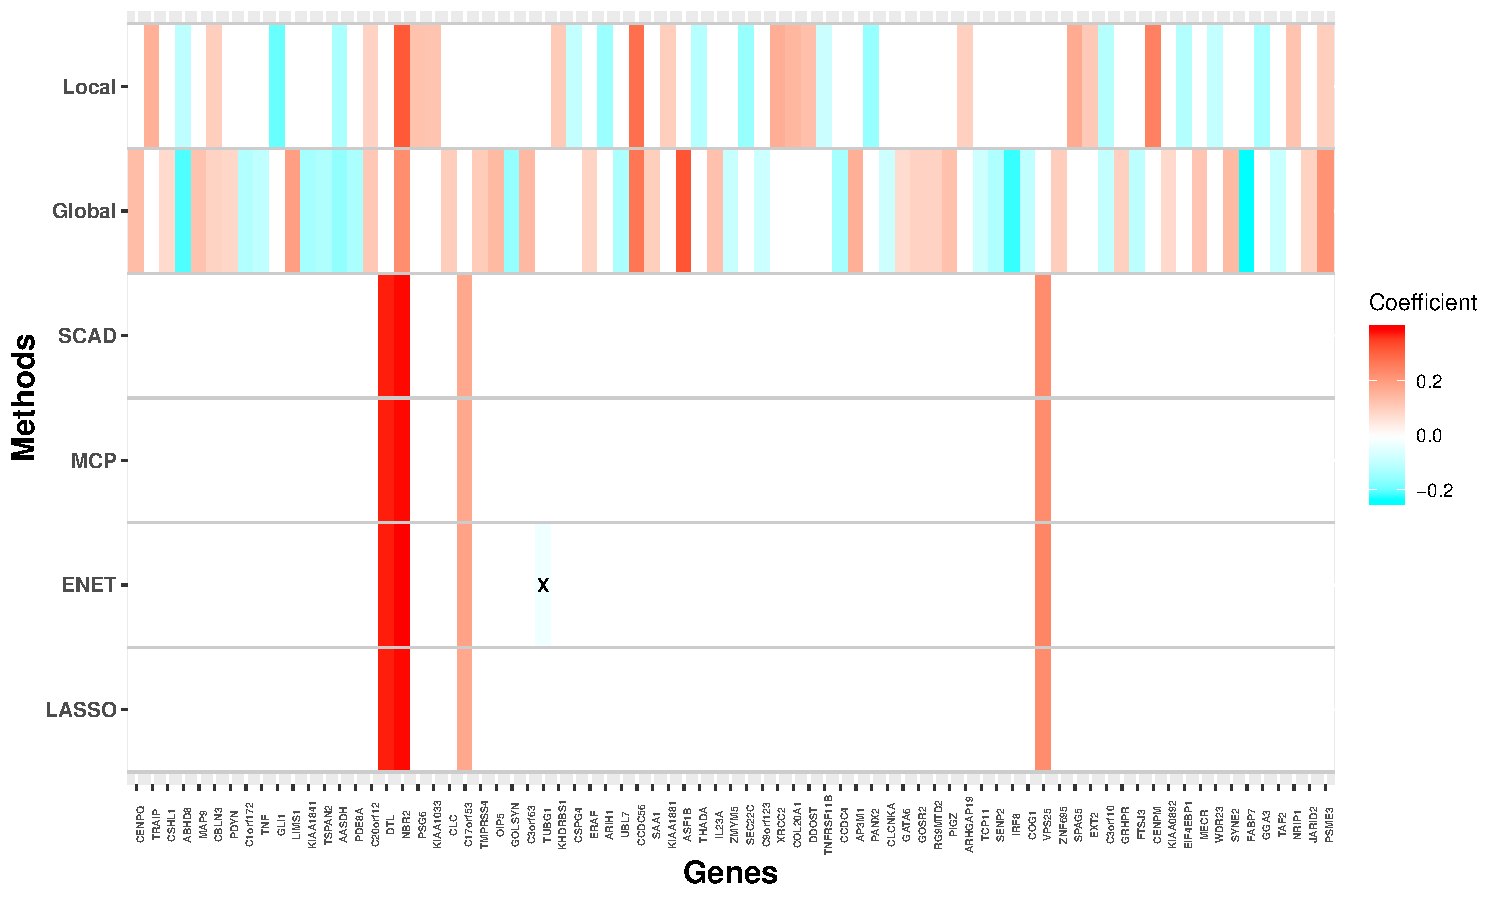
\includegraphics[width=\linewidth]{Heatmap.pdf}
  \caption{Heap map}
  \label{fig:heatmap}
\end{figure}

\begin{figure}
  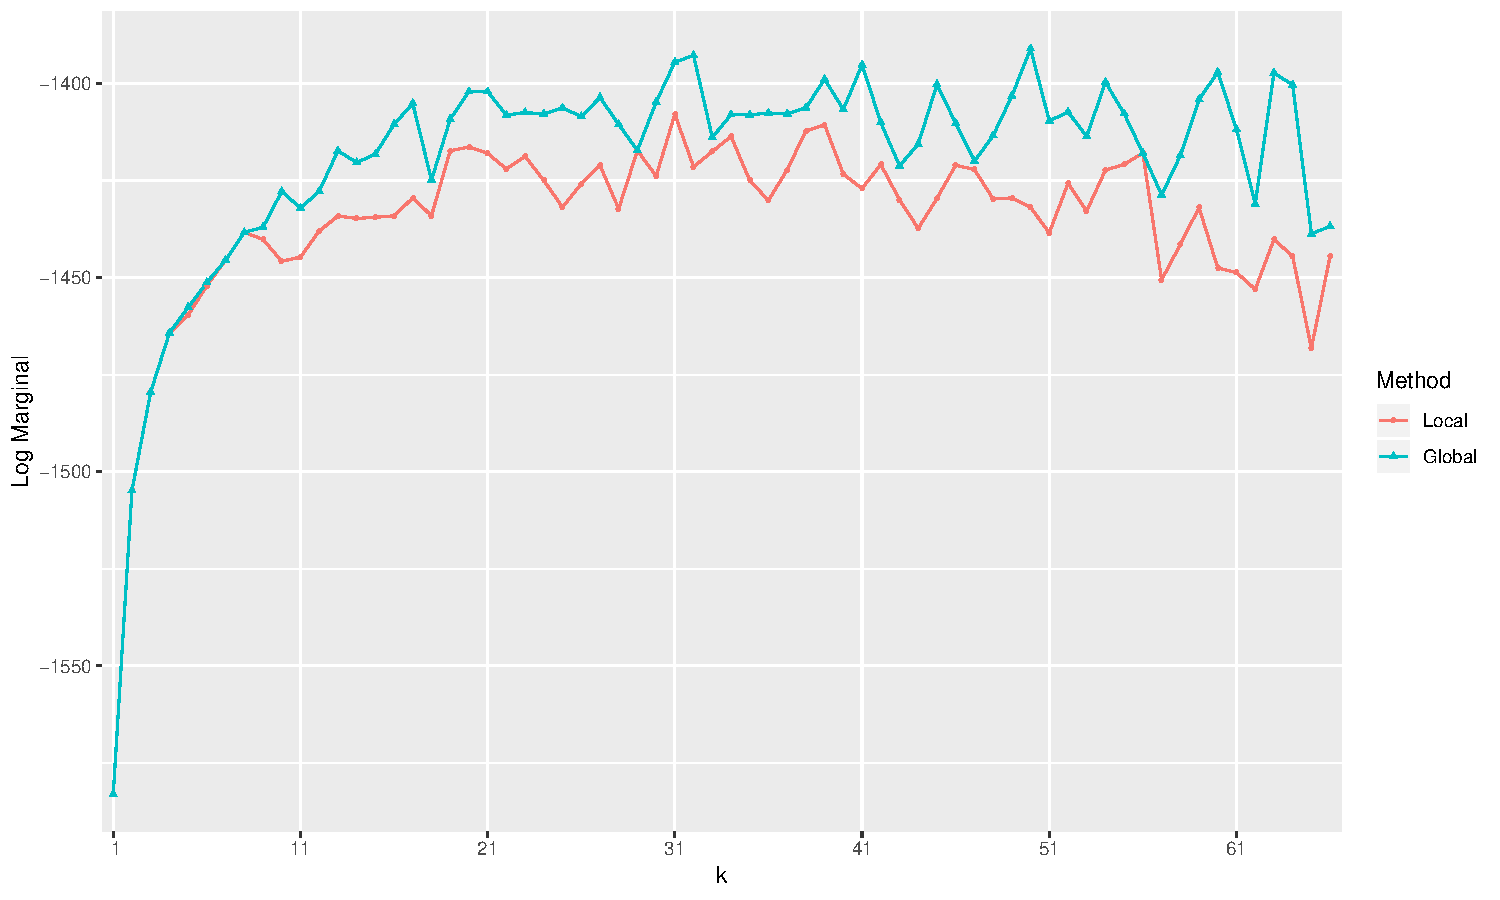
\includegraphics[width=\linewidth]{Log_marginal.pdf}
  \caption{Logmarginal}
  \label{fig:Logmarginal}
\end{figure}




\newpage
\appendix
\section{Proof}\label{app:01}
\begin{proof}[Proof of Theorem \ref{thm:1}] Let $\tilde{\bg}^{(i)}$ be the best subset of size $k$ updated by the $i^{th}$ iteration. Then,
$$\tilde{\ueta}^{(i)}=\arg\max_{\ueta  \in \mathcal{N}_+(\tilde{\bg}^{(i)}  ) } m(\uy|\bg)\quad \text{and}\quad \tilde{\bg}^{(i+1)} = \arg\max_{\bg  \in \mathcal{N}_-(\tilde{\ueta}^{(i)} ) } m(\uy|\bg).$$
Due to the fact that $\tilde{\bg}^{(i)} \in \mathcal{N}_-(\tilde{\ueta}^{(i)} ) $, we have
$$m(\uy|\tilde{\bg}^{(i)} ) \leq m(\uy|\tilde{\bg}^{(i+1)}).$$
From Bayes' theorem, this implies 
$$\pi(\tilde{\bg}^{(i)}|\uy ) \leq \pi(\tilde{\bg}^{(i+1)}|\uy),$$
which proves our first statement.
Since the number of all possible $\bg$ satisfying $|\bg|=k $ is finite, the algorithm terminates in a finite number of iterations and this completes our proof.
\end{proof}
\section{Calculation of \eqref{eq:app:1}}\label{app:1}
\begin{eqnarray}
\pi(\bg^{+i}|\uy,\bg)&\propto& \frac{(\tau^{-1})^{(k+1)/2}}{|\uX_{\bg^{+i}}^{\T}\uX_{\bg^{+i}}+\tau^{-1}I_{k+1} |^{1/2} } \left(\uy^{\T}\uH_{\bg^{+i}}\uy+b_{\sigma}\right)^{-\frac{a_{\sigma}+n}{2} } \mathbb{I}\left\{|\bg^{+i}|=k+1 \right\}\nonumber\\
&\propto&|\uX_{\bg^{+i}}^{\T}\uX_{\bg^{+i}}+\tau^{-1}I_{k+1} |^{-1/2}\left(\uy^{\T}(\uH_\bg-\frac{\uH_\bg \ux_i \ux_i
  ^{\T}\uH_\bg } {\tau^{-1}+\ux_i^{\T}\uH_\bg \ux_i })\uy+b_{\sigma}\right)^{-\frac{a_{\sigma}+n}{2}}\nonumber\\
&=&| \uX_\bg^{\T}\uX_\bg+\tau^{-1}\uI_{k}|^{-1/2} \left(\tau^{-1}+\ux_i^{\T}\uH_\bg \ux_i\right)^{-1/2}\left(\uy^{\T}(\uH_\bg-\frac{\uH_\bg \ux_i \ux_i^{\T}\uH_\bg } {\tau^{-1}+\ux_i^{\T}\uH_\bg \ux_i })\uy+b_{\sigma}\right)^{-\frac{a_{\sigma}+n}{2}}\nonumber\\
&\propto& \left[\uy^{\T}\uH_{\bg}\uy-\frac{(
 	\ux_i^{\T}\uH_{\bg}\uy)^2}{\tau^{-1}+\ux_i^{\T}\uH_{\bg} \ux_i }+b_{\sigma}\right]^
 {-\frac{a_{\sigma}+n}{2}}(\tau^{-1}+\ux_i^{\T}\uH_{\bg} \ux_i)^{-1/2}
\end{eqnarray}
The second proportion holds by Lemma 1 in \ref{lm:1} and the equation holds by Lemma 4.1 in \ref{lm:4.1}
\section{Calculation of \eqref{eq:app:2}}\label{app:2}

The details are shown in Appendix \ref{app:2}.
\begin{eqnarray}
&&\pi(\bg^{*-\ell}|\uy,\bg^*) \nonumber \\
&\propto&\frac{(\tau^{-1})^{k/2}}{|\uX_{\bg^{*-\ell}}^{\T}\uX_{\bg^{*-\ell}}+\tau^{-1}I_{k} |^{1/2} } \left(\uy^{\T}\uH_{\bg^{*-\ell}}\uy+b_{\sigma}\right)^{-\frac{a_{\sigma}+n}{2} } \mathbb{I}\left\{|\bg^{*-\ell}|=k \right\}\nonumber\\
&\propto& |\uX_{\bg^{*-\ell}}^{\T}\uX_{\bg^{*-\ell}}+\tau^{-1}I_{k}|^{-1/2}\left(\uy^{\T}(\uH_{\bg^*}+\frac{\uH_{\bg^*} \ux_{\ell} \ux_{\ell}^{\T}\uH_{\bg^*} } {\tau^{-1}-\ux_{\ell}^{\T}\uH_{\bg^*} \ux_{\ell} })\uy+b_{\sigma}\right)^{-\frac{a_{\sigma}+n}{2}} \nonumber \\
&=& |\uX_{\bg^*}^{\T}\uX_{\bg^*}+\tau^{-1}\uI_{k+1}|^{-1/2} (\tau^{-1}-\ux_\ell^{\T}\uH_{\bg^*} \ux_\ell)^{-1/2}\left[\uy^{\T}\uH_{\bg^*}\uy+\frac{(\ux_\ell^{\T}\uH_{\bg^*}\uy)^2}{\tau^{-1}-\ux_\ell^{\T}\uH_{\bg^*} \ux_\ell }+b_{\sigma}\right]^{-\frac{a_{\sigma}+n}{2}} \nonumber \\
&\propto& \left[\uy^{\T}\uH_{\bg^*}\uy+\frac{(\ux_\ell^{\T}\uH_{\bg^*}\uy)^2}{\tau^{-1}-\ux_\ell^{\T}\uH_{\bg^*} \ux_\ell }+b_{\sigma}\right]^
  {-\frac{a_{\sigma}+n}{2}}(\tau^{-1}-\ux_\ell^{\T}\uH_{\bg^*} \ux_\ell)^{-1/2},
\end{eqnarray}
\section{Lemmas}\label{app:3}
\begin{lemma}\label{lem:1}
Let $\uX=UDV^{\T}$. We have
\begin{eqnarray}\label{lm:5.1}
	|\uX^{\T}\uX+\tau^{-1}\uI_p|
	&=&|VD^{\T}U^{\T}UDV^{\T}+\tau^{-1}VV^{\T}|\nonumber\\
	&=&|VD^{\T}DV^{\T}+V\tau^{-1}\uI_pV^{\T}|\nonumber\\
	&=&|V(D^{\T}D+\tau^{-1}\uI_p)V^{\T}|\nonumber\\
	&=&|V||D^{\T}D+\tau^{-1}\uI_p||V^{\T}|\nonumber\\
	&=&|VV^{\T}||D^{\T}D+\tau^{-1}\uI_p|\nonumber\\
	&=&|D^{\T}D+\tau^{-1}\uI_p|\nonumber\\
	&=&\prod_{j=1}^{p}(d_j^2+\tau^{-1})
\end{eqnarray}
where $d_j$ is $j^{th}$ diagonal element of $D$. Also, we have
\begin{eqnarray}\label{lm:5.2}
	&&\uy^{\T}\uX(\uX^{\T}\uX+\tau^{-1}\uI_p)^{-1}\uX^{\T}\uy\nonumber\\
	&=& \uy^{\T}UDV^{\T}(VD^{\T}U^{\T}UDV^{\T}+V\tau^{-1}\uI_pV^{\T})^{-1}
	VD^{\T}U^{\T}\uy \nonumber\\
	&=& \uy^{\T}UDV^{\T}(V(D^{\T}D+\tau^{-1}\uI_p)V^{\T})^{-1}
	VD^{\T}U^{\T}\uy \nonumber\\
	&=& \uy^{\T}UD(D^{\T}D+\tau^{-1}\uI_p)^{-1}D^{\T}U^{\T}\uy \nonumber\\
	&=& \uy^{\T}UD(\diag(d_j^2+\tau^{-1}))^{-1}D^{\T}U^{\T}\uy \nonumber\\
	&=& \uy^{\T}U\diag\left(\frac{d_j^2}{d_j^2+\tau^{-1}}\right)U^{\T}\uy \nonumber\\
	&=& \sum_{j}\frac{d_j^2z_j^2}{d_j^2+\tau^{-1} }
	\end{eqnarray}
where $z_j$ is the $j^{th}$ component of $U^{\T}\uy$.
\end{lemma}



\bibliographystyle{chicago}
\bibliography{ref}
\end{document}
